
\documentclass[11pt]{article}


\setlength{\oddsidemargin}{0.0in}
\setlength{\evensidemargin}{0.0in}
\setlength{\topmargin}{0.0in}
\setlength{\topskip}{0.5in}
\setlength{\headheight}{0.5in}
\setlength{\headsep}{0in}
\setlength{\textwidth}{6.5in}
\setlength{\textheight}{8.0in}
\setlength{\parindent}{0in}
\setlength{\parskip}{0.1in}

\setcounter{secnumdepth}{4}
\setcounter{tocdepth}{4}

% \usepackage{times}
\usepackage{fancyvrb}
\usepackage{relsize}
\usepackage{hyperref}
\usepackage{graphicx}
\usepackage{color}
\usepackage{listings}

% theorems, etc.
\usepackage{amsmath}
\newtheorem{theorem}{Theorem}
\newcommand{\BlackBox}{\rule{1.5ex}{1.5ex}}  % end of proof
\newenvironment{proof}{\par\noindent{\bf Proof\ }}{\hfill\BlackBox\\[2mm]}
\newtheorem{lemma}[theorem]{Lemma}
\newtheorem{proposition}[theorem]{Proposition}
\newtheorem{remark}[theorem]{Remark}
\newtheorem{corollary}[theorem]{Corollary}
\newtheorem{definition}[theorem]{Definition}
\newtheorem{conjecture}[theorem]{Conjecture}
\newtheorem{axiom}[theorem]{Axiom}

% for problem sets, each problem automatically numbered
\newcounter{problemnum}
\newcommand{\oneproblem}
   { \stepcounter{problemnum} {\bf \arabic{problemnum}}. } 
\newcommand{\startproblemset}
   { \bigskip {\bf\large Exercises} \setcounter{problemnum}{0} }

\lstset{language=r}
\lstset{
    literate={~} {$\sim$}{1}
}
\lstset{basicstyle=\ttfamily}


 

\begin{document} 

\title{Mixture and Hidden Markov Models}
\author{Norman Matloff \\
   Department of Computer Science \\
   University of California, Davis}

\maketitle

The notion of \textit{mixture distributions} is a classical
probabilistic concept, and arises frequently in applications.  The field
of \textit{Hidden Markov Models} (HMMs) is more ``recent'' on the scale
of this area, and have very interested applications, such as in
bioinformatics and language processing.

As there is a natural connection of mixture models (MMs) to HMMs, we
present both here.  

\section{First Motivating Example:  Old Faithful Geyser}

The data here consist of waiting times between eruptions of the famous
Old Faithful geyser in the US' Yellowstone National Park.  The dataset
here is \textbf{faithful}, a built-in dataset in R.

A histogram, obtained via 

\begin{lstlisting}
> hist(faithful$waiting)
\end{lstlisting}

and shown in Figure \ref{faithfulhist}, seems to suggest that the
waiting time distribution is a mixture of two normally distributed random
variables.  This seems even more plausible if we use R's
\textbf{density} function, as in Figure \ref{faithfulhistsmooth}.

This has led to many physical theories over the years.  For instance,
are there actually (in whatever sense) two geysers underground, erupting 
at random times according to two separate normal distributions?
Actually, rather elaborate physical models have been
developed.\footnote{E.g. O'Hara and Esawi, 
Model for the eruption of the Old Faithful geyser, Yellowstone National
Park, \textit{GSA Today}, June 2013.} 

\subsection{Second Motivating Example:  Network Noise}

Suppose we have a network line that is known to occasionally be
noisy, and that during noisy periods all bits will be corrupted in such
a way that the probability of a 0, which is 0.5 in the original
transmitted data, is 0.20 during noisy periods.  Suppose that on average
10\% of the bits arrive during noise periods.

\section{``Hidden'' States}

For the purposes of the discussion here, let's take as our model the
``two underground geysers'' version.  Our \textit{hidden}, i.e.\ unknown, state
here will be the identity of the currently erupting geyser, Geyser 1 or
Geyser 2.  Our \textit{observed} state is the waiting time between
eruptions of any kind.

In the network example, the hidden state is whether we are currently in
a clear period (coded 1) or a noisy period (coded 2).  The observed
state is the actual received bit.

A complicating factor in the first example is that, if indeed there are
two geysers, we observe the minimum of two geyser times.  So,
from this point onward, we will focus on the second motivating model,
that of the noisy network.

\section{``Time''}

In some applications, time is really time.  If our data is stock price,
say, we have Day 1, Day 2, Day 3 and so on.  In other applications,
``time'' is an index, such at Bit 1, Bit 2, Bit 3 etc.

\section{Conditional Probabilities of Observed Values}

Let $S_i$ denote the hidden state at time $i$, 
and let $Y_i$ denote the corresponding observed value.  A key ingredient
in the analysis will be expressions of the form

\begin{equation}
P(Y_i = w | S _i = v)
\end{equation}

If $Y$ is continuous rather than discrete, the above expression would be
something like

\begin{equation}
f_{Y|S} (w,v) 
\end{equation}

where $f_{Y|S}$ is the conditional density of $Y$ given $S$.

These conditional distribution quantities are then used to estimate
model parameters, as we will see below.

\section{Mixture Models vs.\ HMMs}

Both types of models have hidden and observed states.  But HMMs add an
extra aspect:  We model the probabilities of going from one state to
another in one unit of time.

\begin{figure}[tb]
\centerline{
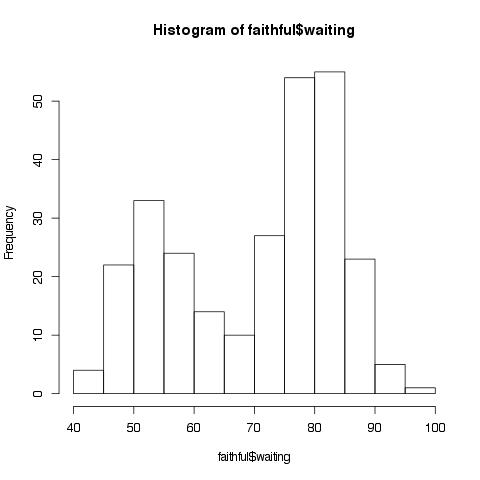
\includegraphics[width=3.0in]{Faithful.jpg}
}
\caption{Old Faithful waiting times}
\label{faithfulhist}
\end{figure}

\begin{figure}[tb]
\centerline{
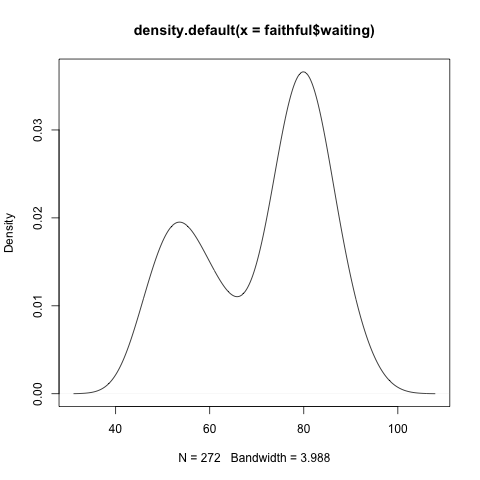
\includegraphics[width=3.0in]{FaithfulSmooth.png}
}
\caption{Old Faithful waiting times, Smoothed}
\label{faithfulhistsmooth}
\end{figure}

\section{Mixtures}

Consider random variables $X_1,...,X_k$, with cumulative distribution
functions $F_{X_i}$ (not necessarily independent), and let $c_i, ~
i=1,...,k$ be nonnegative numbers whose sum is 1.  Define the random
variable $M$ to take on the value $X_i$ with probability $c_i$,
$i=1,...,k$.  Then we say that $M$ has a mixture distribution.

Note that

\begin{equation}
F_{M}(t) = \sum_{i=1}^k c_i F_{X_i}(t)
\end{equation}

Similar relations hold for probability mass functions ($X_i$ discrete)
and density functions ($X_i$ continuous).

\subsection{Use of the mixtools Package}

I tried initial guesses of means and standard deviations from the
appearance of the histogram, and used equal weights for my initial
guesses in that aspect:

\begin{lstlisting}
> mixout <- normalmixEM(faithful$waiting,lambda=0.5,mu=c(55,80),sigma=10,k=2)
number of iterations= 9 
> str(mixout)
List of 9
 $ x         : num [1:272] 79 54 74 62 85 55 88 85 51 85 ...
 $ lambda    : num [1:2] 0.361 0.639
 $ mu        : num [1:2] 54.6 80.1
 $ sigma     : num [1:2] 5.87 5.87
 $ loglik    : num -1034
 $ posterior : num [1:272, 1:2] 1.02e-04 1.00 4.12e-03 9.67e-01 1.21e-06
...
  ..- attr(*, "dimnames")=List of 2
  .. ..$ : NULL
  .. ..$ : chr [1:2] "comp.1" "comp.2"
 $ all.loglik: num [1:10] -1085 -1051 -1037 -1034 -1034 ...
 $ restarts  : num 0
 $ ft        : chr "normalmixEM"
 - attr(*, "class")= chr "mixEM"
\end{lstlisting}

So, the estimate from EM is that about 36\% of the eruptions are of Type
1, etc.  Interesting, when I tried it without my own initial guesses,

\begin{lstlisting}
mixout <- normalmixEM(faithful$waiting,k=2)
\end{lstlisting}

the results were the same, so it seems to be a fairly stable model here.

By the way, since we are working with a hidden variable M here---in
fact, we are merely postulating that it exists---how do we check this
assumption?  We'll return to this general idea of model fitting in
Chapter \ref{chap:mod}.

\section{The Old Trick Coin Example, Updated}
\label{oldtrick}

Recall the trick coin example in Section \ref{caution}.  Let's look at a
somewhat different version.

Suppose we have a large box of coins of two types. One type has
probability p of heads, the other probability q of heads. A proportion r
of the coins is of the first type. We reach into the box, choose a coin
at random, and toss that coin 10 times, resulting in N heads. What is
the distribution of N?

Since N is discrete, the distribution is described by its pmf, which is

\begin{equation}
\label{mixbinom}
p_N(k) = r \binom{10}{k} p^k (1-p)^{10-k} +
(1-r) \binom{10}{k} q^k (1-q)^{10-k}
\end{equation}

You can see why this is called a {\it mixture} model. The above pmf is a
mixture of two binomial pmfs, with mixing proportions r and 1-r.

\section{General Mixture Distributions}
\label{genmix}

The general definition is rather abstract.  Let's first restrict it to
discrete outputs:

\begin{definition} Let $\{g_t\}_{t \in A}$ be a collection of pmfs, and
let M be a random variable taking values in A.  Consider discrete and
continuous cases for M, as follows.  The {\bf mixture distribution} of
the $g_t$ with weights given by the distribution of M is defined as
follows:

\begin{itemize}

\item M is discrete:  The mixture distribution is the pmf\footnote{The
reader should verify that H does qualify as a pmf, i.e. it consists of
numbers in [0,1] that sum to 1.}

\begin{equation}
\label{hsum}
h = \sum_{i \in A} p_M(i) ~ g_i
\end{equation}

\item M is continuous:  The mixture distribution has the pmf 

\begin{equation}
\label{continmix}
h(u) = \int_{t \in A} f_M(t)~  g_t(u) ~ dt
\end{equation}

\end{itemize}

{\bf For continuous outcomes, replace ``pmf'' by ``density'' everywhere
above.}

\end{definition}

\vskip 0.5in

Actually, the definition isn't so abstract after all.  A random variable
Y having pmf or density h arises first of the random variable M, and then if M
= i, getting Y randomly from the distribution $g_i$.  A ``notebook''
analysis would have columns for both M and Y.

In other words, the pmf of Y is a weighted average of the $g_i$, with
weights being the pmf of M.  Note that this implies that the weights
most be nonnegative and sum to 1.\footnote{Some readers may recognize
this as a {\bf convex combination}.}

As noted, the above definition is pretty abstract, but it can be readily
grasped by considering the above trick coin example.  Here,
% (\ref{caution}) is (\ref{hsum}), with

\begin{itemize}

\item $Y = N$

\item A = \{0,1\}

\item $p_M(0) = p_M(1) = 0.5$

\item $g_0$ = the pmf for B(i,0.1)

\item $g_1$ = the pmf for B(i,0.9)

\end{itemize}

Mixture distributions occur in a surprisingly wide variety of
applications, and thus this material should be mastered.  It is somewhat
difficult at first, but if you always keep concrete examples such as the
trick coin problem in mind, it is not bad at all.

By the way, there is nothing in the above definition that limits the
$G_i$ and H to be for scalar random variables.  They could all be
bivariate, for instance (though of course they all have to be of the
same dimension.)

\section{Generating Random Variates from a Mixture Distribution}

One way to get additional insight on mixture distributions is to think
about how to simulate them.  For instance, consider the trick coin problem.
The following R code simulates $X_i$:

\begin{lstlisting}
rxi <- function(i) {
   m <- sample(0:1,1)
   p <- if (M ==0) 0.1 else 0.9
   rbinom(1,i,p)
}
\end{lstlisting}

In general:

\begin{itemize}

\item We first generate M.

\item Then we generate a random variable from the pmf $G_M$.

\end{itemize}

Various examples of mixture distributions will be presented in this
chapter.  But first, we need to develop some machinery.

% \section{Conditional Distributions}
% 
% The key to good probability modeling and statistical analysis is to
% understand conditional probability.  The issue arises constantly.
% 
% \subsection{Conditional Pmfs and Densities}
% 
% First, let's review:  In many repetitions of our ``experiment,'' P(A) 
% is the long-run proportion of the time that A occurs.  By contrast,
% P(A$|$B) is the long-run proportion of the time that A occurs, {\it
% among those repetitions in which B occurs.}  Keep this in your mind at
% all times.
% 
% Now we apply this to pmfs, densities, etc.  We define the conditional
% pmf as follows for discrete random variables X and Y:
% 
% \begin{equation}
% \label{discrcond}
% p_{Y|X}(j|i) = P(Y = j | X = i) = \frac{p_{X,Y}(i,j)}{p_X(i)}
% \end{equation}
% 
% By analogy, we define the conditional density for continuous X and Y:
% 
% \begin{equation}
% \label{contcond}
% f_{Y|X}(t|s) = \frac{f_{X,Y}(s,t)}{f_X(s)}
% \end{equation}
% 
% \subsection{Conditional Expectation}
% 
% Conditional expectations are defined as straightforward extensions of
% (\ref{discrcond}) and (\ref{contcond}):
% 
% \begin{equation}
% E(Y|X=i) = \sum_{j} j p_{Y|X}(j|i) 
% \end{equation}
% 
% \begin{equation}
% E(Y | X = s) = \int_{t} t f_{Y|X}(t|s) ~ dt
% \end{equation}

\section{A Useful Tool:  the Law of Total Expectation}
\label{lte}

Let's put the mixture distribution issue aside for a moment, to discuss
a tool that is useful both in mixture models and elsewhere.

The notion of iterated expectation, which was introduced in Sections
\ref{iterexp} and \ref{adamscontin}, is an extremely important
tool for the analysis of mixture distributions.  We first need to extend
our earlier definitions somewhat.

Again, this will seem rather abstract at first, but you'll see that it
is a great convenience.

\subsection{Conditional Expected Value As a Random Variable}

For random variables Y and W, and an event, say W = t, the quantity
E(Y$|$W = t) is the long-run average of Y, among the times when W = t
occurs.  

Note several things about the expression E(Y$|$W = t):

\begin{itemize}

\item The item to the left of the $|$ symbol is a {\it random variable} (Y).

\item The item on the right of the $|$ symbol is an {\it event} (W = t).

\item The overall expression evaluates to a constant.

\end{itemize}

By contrast, for the quantity E(Y$|$W) to be defined shortly,
it is the case that:

\begin{itemize}

\item The item to the left of the $|$ symbol is a random variable (Y).

\item The item to the right of the $|$ symbol is a random variable (W).

\item The overall expression itself is a random variable, not a constant.

\end{itemize}

It will be very important to keep these differences in mind.

Consider the function g(t) defined as\footnote{Of course, the t is just
a placeholder, and any other letter could be used.} 

\begin{equation}
\label{thisisg}
g(t)=E(Y|W=t)
\end{equation}

In this case, the item to the right of the $|$ is an event, and thus
g(t) is a constant (for each value of t), not a random variable.

\begin{definition}

Define g() as in (\ref{thisisg}).  Form the new random variable Q =
g(W).  Then the quantity E(Y$|$W) is defined to be Q. 

\end{definition}

(Before reading any further, re-read the two sets of bulleted items
above, and make sure you understand the difference between E(Y$|$W=t)
and E(Y$|$W).)

One can view E(Y$|$W) as a projection in an abstract vector space.  This
is very elegant, and actually aids the intuition.  If (and only if) you
are mathematically adventurous, read the details in Section
\ref{elegant}.

\subsection{Famous Formula: Theorem of Total Expectation}

An extremely useful formula, given only scant or no mention in
most undergraduate probability courses, is 

\begin{equation}
\label{itex}
E(Y)=E[E(Y|W)]
\end{equation}

for any random variables Y and W (for which the expectations are
defined).  

The RHS of (\ref{itex}) looks odd at first, but it's merely E[g(W)];
since Q =  E(Y$|$W) is a random variable, we can certainly ask what its
expected value is.

Equation (\ref{itex}) is a bit abstract.  It's a very useful
abstraction, enabling streamlined writing and thinking about the
probabilistic structures at hand.  Be sure to review the intuitive
explanation following (\ref{adamsdiscrete}) before continuing.

% Still, you may find it helpful to
% consider the case of discrete W, in which (\ref{itex}) has the more
% concrete form
% 
% \begin{equation}
% \label{itexdiscrete}
% EY = \sum_{i} P(W=i) \cdot E(Y|W=i)
% \end{equation}
% 
% To see this intuitively, think of measuring the heights and weights of
% all the adults in Davis.  Say we measure height to the nearest inch, so
% that height is discrete.  We look at all the adults in Davis who are 72
% inches tall, and write down their mean weight.  Then we write down the
% mean weight of all adults of height 68.  Then we write down the mean
% weight of all adults of height 75, and so on.  Then (\ref{itex}) says
% that if we take the average of all the numbers we write down---the
% average of the averages---then we get the mean weight among {\it all}
% adults in Davis.  
% 
% Note carefully, though, that this is a {\it weighted} average.  If for
% instance people of height 69 inches are more numerous in the population,
% then their mean weight will receive greater emphasis in over average of
% all the means we've written down.  This is seen in (\ref{itexdiscrete}),
% with the weights being the quantities P(W=i).

% The relation (\ref{itex}) is proved in the discrete case in Section
% \ref{proveitex}.

\subsection{Properties of Conditional Expectation and Variance}

Conditional expected value is still expected value, and thus still has
the usual properties of expected value.  In particular,

\begin{equation}
E(aU + bV ~|~ W) = a E(U ~|~ W) + b E(V ~|~ W)
\end{equation}

for any constants {\it a} and $b$.  The same is true for variance, e.g.

\begin{equation}
Var(aU | W) = a^2 Var(U ~|~ W)
\end{equation}

for any constants $a$, and 

\begin{equation}
Var(U + V ~|~ W) = Var(U ~|~ W) + Var(V ~|~ W)
\end{equation}

if U and V are {\it conditionally independent}, given W.

The reason for all this is simple.  Consider the discrete case, for
convenience.  As seen in (\ref{a}), E(Z) is a weighted average of the
values of Z, with the weights being the values of $p_Z$:

\begin{equation}
EZ = \sum_c c p_Z(c)
\end{equation}

But $E(Z | T)$ is simply another weighted average, with the weights
being the conditional distribution of Z given T:

\begin{equation}
E(Z | T) = \sum_c c p_{Z|T}(c)
\end{equation}

Note that (continuing the discrete case)

\begin{equation}
p_{Z|T=r}(c) =
\frac{P(Z = c, T = r)}{P(T = r)}
\end{equation}

All this extends to variance, since it too is defined in terms of
expected value, in (\ref{vardef}).  So,

\begin{equation}
Var(Z | T) = E\{[Z - E(Z|T)]^2\}
\end{equation}

And of course, if the variables above are continuous, just replace pmfs
for densities, and sums by integrals.

\subsection{Example:  More on Flipping Coins with Bonuses}

Recall the situation of Section \ref{bonusflip}:  A game involves
flipping a coin k times.  Each time you get a head, you get a bonus
flip, not counted among the k.  (But if you get a head from a bonus
flip, that does not give you its own bonus flip.) Let Y denote the
number of heads you get among all flips, bonus or not.   We'll compute
EY.

Let

\begin{eqnarray}
W &=& \textrm{ number of heads from nonbonus flips} \\ 
  &=& \textrm{ number of bonus flips} 
\end{eqnarray}

This is a natural situation in which to try the Theorem of Total
Expectation, conditioning on Y.  Reason as follows:

Y-W is the number of heads obtained from the bonus flips.  Given W, the
random variable Y-W has a binomial distribution with parameters W and
0.5, so 

\begin{equation}
E(Y-W ~|~ W) = 0.5 W
\end{equation}

Then from (\ref{itex}),

\begin{eqnarray}
EY &=& E[E(Y ~|~ W)] \\ 
&=& E \left [E ( \{ Y-W \} + W ~|~ W ) \right ] \\
&=& E \left [E (Y-W | W) + E(W ~|~ W ) \right ] \\
&=& E \left [ 0.5W + W \right ] \\
&=& 1.5 EW \\
&=& 0.75 k,
\end{eqnarray}

that last result coming from the fact that W itself has a binomial
distribution with k trials and success probability 0.5.

Now here is the point:  We could have used (\ref{adamsdiscrete}) above.
But our use of (\ref{itex}) really streamlined things.  If we had
invoked (\ref{adamsdiscrete}), we would have had a messy sum, with
binomial pmf expressions and so on.  By using (\ref{itex}), we avoided
that, a big win.

\subsection{Example:  Trapped Miner}
\label{trappedminer}

This rather whimsical example is adapted from \textit{Stochastic
Processes,} by Sheldon Ross, Wiley, 1996.

A miner is trapped in a mine, and has a choice of three doors.  Though
he doesn't realize it, if he chooses to exit the first door, it will
take him to safety after 2 hours of travel.  If he chooses the second
one, it will lead back to the mine after 3 hours of travel. The third
one leads back to the mine after 5 hours of travel. Suppose the doors
look identical, and if he returns to the mine he does not remember which
door(s) he tried earlier. What is the expected time until he reaches
safety?

The answer turns out to be 10.  This is no accident, as 2+3+5 = 10.
This was discovered on an intuitive basis (shown below) by UCD grad
student Ahmed Ahmedin.  Here is how we can derive the answer, using
(\ref{itex}):

Let Y be the time needed to reach safety, let N denote the total
number of attempts the miner makes before escaping (including the
successful attempt at the end), and let $U_i$ denote the time spent
traveling during the $i^{th}$ attempt, i = 1,...,N.  Then

\begin{eqnarray}
EY &=& E(U_1+...,+U_N) \\ 
&=& E \left [ E(U_1+...+U_N | N) \right ] 
\end{eqnarray}

Note carefully that the expression $U_1+...+U_N$ not only has random
terms, but also the {\it number} of terms, N, is random.  So,
technically, we cannot use (\ref{aubv}) or its extension to multiple
terms.  But by conditioning on N, we are back in the situation of a
fixed number of terms, and can proceed.

Given N, each of $U_1,...,U_{N-1}$ takes on the values 3 and 5, with
probability 0.5 each, while $U_N$ is the constant 2.  Thus

\begin{equation}
E(U_1+...,+U_N | N) = (N-1) \frac{3+5}{2} + 2 = 4N - 2
\end{equation}

N has a geometric distribution with success probability p = 1/3, so EN =
3.  Putting all this together, we have

\begin{eqnarray}
EY &=& E(U_1+...,+U_N) \\
&=& E\left [ E(U_1+...,+U_N | N) \right ] \\
&=& E(4N - 2) = 10
\end{eqnarray}

If 2, 3 and 5 were replaced by {\it a}, {\it b} and {\it c}, the result
would turn out to be a+b+c.  Intuitively:  It takes an average of 3
attempts to escape, with each attempt having mean time of (a+b+c)/3, so
the mean time overall is a+b+c.

Here is a different derivation (the one in Ross' book):

Let W denote the number of the door chosen (1, 2 or 3) on the first try.
Then let us consider what values E(Y$|$W) can have. If W = 1, then Y =
2, so

\begin{equation}
E(Y|W=1)=2
\end{equation}

If W = 2, things are a bit more complicated. The miner will go on a
3-hour excursion, and then be back in his original situation, and thus
have a further expected wait of EY, since ``time starts over.''  In
other words,

\begin{equation}
E(Y|W=2)=3+EY
\end{equation}


Similarly, 

\begin{equation}
E(Y|W=3)=5+EY
\end{equation}

In summary, now considering the \textit{random variable} E(Y$|$W), we have

\begin{equation}
Q=E(Y|W)=\left\{ \begin{array}{rl}
2, & w.p.\frac{1}{3}\\
3+EY, & w.p.\frac{1}{3}\\
5+EY, & w.p.\frac{1}{3}
\end{array}\right. 
\end{equation}

where ``w.p.'' means ``with probability.'' So, using (\ref{itex}) we have

\begin{equation}
EY=EQ=2\times \frac{1}{3}+(3+EY)\times \frac{1}{3}+(5+EY)\times \frac{1}{3}=\frac{10}{3}+\frac{2}{3}EY
\end{equation}

Equating the extreme left and extreme right ends of this series of equations,
we can solve for EY, which we find to be 10.


It is left to the reader to see how this would change if we assume that the
miner remembers which doors he has already hit.

\subsection{Example:  Analysis of Hash Tables}

(Famous example, adapted from various sources.)

Consider a database table consisting of m cells, only some of which are
currently occupied. Each time a new key must be inserted, it is used in
a hash function to find an unoccupied cell. Since multiple keys can map to
the same table cell, we may have to probe multiple times before finding
an unoccupied cell.

We wish to find E(Y), where Y is the number of probes needed to insert a
new key.  One approach to doing so would be to condition on W, the
number of currently occupied cells at the time we do a search.  After
finding E(Y$|$W), we can use the Theorem of Total Expectation to find
EY.  We will make two assumptions (to be discussed later):

\begin{itemize}

\item [(a)] Given that W = k, each probe will collide with an existing
cell with probability k/m, with successive probes being independent.

\item [(b)] W is uniformly distributed on the set 1,2,...,m, i.e. P(W =
k) = 1/m for each k.

\end{itemize}

To calculate E(Y$|$W=k), we note that given W = k, then Y is the
number of independent trials until a ``success'' is reached, where
``success'' means that our probe turns out to be to an unoccupied cell.
This is a {\bf geometric} distribution, i.e.

\begin{equation}
P(Y = r | W = k) = {(\frac{k}{m})}^{r-1} (1-\frac{k}{m})
\end{equation}

The mean of this geometric distribution is, from (\ref{eofgeom}),

\begin{equation} 
\frac{1}{1-\frac{k}{m}}
\end{equation}

Then 

\begin{eqnarray}
EY & = & E[E(Y|W)]\\
 & = & \sum ^{m-1}_{k=1}\frac{1}{m}E(Y|W=k)\\
 & = & \sum ^{m-1}_{k=1}\frac{1}{m-k}\\
 & = & 1+\frac{1}{2}+\frac{1}{3}+...+\frac{1}{m-1}\\
 & \approx  & \int_1^m \frac{1}{u} du \\
 & = & \ln(m)
\end{eqnarray}

where the approximation is something you might remember from calculus
(you can picture it by drawing rectangles to approximate the area under
the curve.).

Now, what about our assumptions, (a) and (b)?  The assumption in (a) of
each cell having probability k/m should be reasonably accurate if k is
much smaller than m, because hash functions tend to distribute probes
uniformly, and the assumption of independence of successive probes is
all right too, since it is very unlikely that we would hit the same cell
twice.  However, if k is not much smaller than m, the accuracy will
suffer.

Assumption (b) is more subtle, with differing interpretations.  For
example, the model may concern one specific database, in which case the
assumption may be questionable.  Presumably W grows over time, in which
case the assumption would make no sense---it doesn't even {\it have} a
distribution.  We could instead think of a database which grows and
shrinks as time progresses.  However, even here, it would seem that W
would probably oscillate around some value like m/2, rather than being
uniformly distributed as assumed here.  Thus, this model is probably not
very realistic.  However, even idealized models can sometimes provide
important insights.

% \section{Simulation of Random Vectors}
% 
% Let $X = (X_1,...,X_k)'$ be a random vector having a specified
% distribution.  How can we write code to simulate it?  It is not always
% easy to do this.  We'll discuss a couple of easy cases here, and
% illustrate what one may do in other situations.
% 
% The easiest case (and a very frequenly-occurring one) is that in which
% the $X_i$ are independent.  One simply simulates them individually, and
% that simulates X!
% 
% Another easy case is that in which X has a multivariate normal
% distribution.  We noted in Section \ref{mvnormdens} that R includes the
% function {\bf mvrnorm()}, which we can use to simulate our X here.  The
% way this function works is to use the notion of principle components
% mentioned in Section \ref{datamining}.  We construct Y = AX for the
% matrix A discussed there.  The $Y_i$ are independent, thus easily
% simulated, and then we transform back to X via $X = A^{-1}Y$
% 
% In general, though, things may not be so easy.  For instance, consider
% the distribution in (\ref{tridens}).  There is no formulaic solution
% here, but the following strategy works.  
% 
% First we find the (marginal) density of X.  As in the case for Y shown
% in (\ref{ydens}), we compute
% 
% \begin{equation}
% f_X(s) = \int_{0}^{s} 8st ~ dt = 4s^3
% \end{equation}
% 
% Using the method shown in our unit on continuous probability, Section
% \ref{genrannumgen}, we can simulate X as
% 
% \begin{equation}
% X = F_X^{-1}(W)
% \end{equation}
% 
% where W is a U(0,1) random variable, generated as {\bf runif(1)}.
% Since $F_X(u) = u^4$, $F_X^{-1}(v) = v^{0.25}$, and thus our code to
% simulate X is
% 
% \begin{Verbatim}[fontsize=\relsize{-2}]
% runif(1)^0.25
% \end{Verbatim}
% 
% Now that we have X, we can get Y.  We know that 
% 
% \begin{equation}
% f_{Y|X}(t|S) = \frac{8st}{4s^3} = \frac{2}{s^2} t
% \end{equation}
% 
% Remember, s is considered constant.  So again we use the ``inverse-cdf''
% method here to find Y, given X, and then we have our pair (X,Y).

\subsection{What About the Variance?}
\label{totalvar}

By the way, one might guess that the analog of the Theorem of Total Expectation
for variance is

\begin{equation}
Var(Y)=E[Var(Y|W)]
\end{equation}

\textit{But this is false.} Think for example of the extreme case in which Y
= W. Then Var(Y$|$W) would be 0, but Var(Y) should be nonzero.

The correct formula, called the Law of Total Variance, is

\begin{equation}
\label{bis}
Var(Y)=E[Var(Y|W)]+Var[E(Y|W)]
\end{equation}

Deriving this formula is easy, by simply evaluating both sides of
(\ref{bis}), and using the relation $Var(X) = E(X^2) -(EX)^2$. This
exercise is left to the reader.  See also Section \ref{elegant}.

\section{The EM Algorithm}
\label{emalg}

Now returning to our main topic of mixture models, let's discuss a very
common tool for fitting such models.

Consider again the example in Section \ref{oldtrick}.  Now suppose p, q
and r are all unknown, and we wish to estimate them from data. Say we
will perform the above experiment 50 times, resulting in our data
$N_1,...,N_{50}$ We will estimate p, q and r by applying some method,
say the Method of Moments, Maximum Likelihood or some ad hoc method of
our own, to our data. Each $N_i$ has the distribution seen in $p_N$
above. This is a parametric family, with 3 parameters. (If, say, r is
known, we only have a two-parameter family, and things are easier.)

So, how can we estimate those three parameters?  In Chapter
\ref{chap:est}, we found some general methods for parameter estimation.
Let's look at one of them, Maximum Likelihood Estimators (MLEs).

In (\ref{mixbinom}), the MLE vector 
$(\widehat{p},
  \widehat{q},
  \widehat{r})'$
would be found by maximizing

\begin{equation}
\Pi_{i=1}^n
\left [ r \binom{10}{N_i} p^{N_i} (1-p)^{10-N_i} +
(1-r) \binom{10}{N_i} q^{N_i} (1-q)^{10-N_i}
\right ]
\end{equation}

After taking derivatives, etc., one would end up with a messy, nonlinear
set of equations to solve.  One could try {\bf mle()}, but there is a
better way to get the MLE: the Expection/Maximization (EM) algorithm.
The derivation and ultimate formulas can get quite complex.
Fortunately, R libraries exist, such as {\bf mixtools}, so you can avoid
knowing all the details, as long as you understand the basic notion of a
mixture model.  

\subsection{Overall Idea}

In something like (\ref{hsum}), for instance, one would make initial
guesses for the $p_M(i)$ and then estimate the parameters of the $g_i$.
In the next step, we'd do the opposite---take our current guesses for
the latter parameters as known, and estimate the $p_M(i)$.  Keep going
until convergence.

To make things concrete, recall the trick coin example Section
\ref{oldtrick}.  But change it a little, so that the probabilities of
heads for the two coins are unknown; call them $p_0$ (heads-light coin)
and $p_1$ (heads-heavy coin).  And also suppose that the two coins are
not equally likely to be chosen, so that $p_M()$ is not known; denote
P(M = 1) by q.

Suppose we have sample data, consisting of doing this experiment
multiple times, say by reaching into the box n times and then doing m
flips each time.  We then wish to estimate 3 quantities---q and the two
$p_i$---using our sample data.  

We do so using the following iterative process.  (The account here is
not exactly EM, but captures the spirit of it.) We set up initial
guesses, and iterate until convergence:

\begin{itemize}

\item {\bf E step:} Update guess for q (complicated Bayes Rule equations).

\item {\bf M step:} Using the new guess for q, update the gueses for the
two $p_i$.

\end{itemize}

The details are beyond the scope of this book.\footnote{``M'' in the M
step refers to the Maximum Likelihood method, a special case of the
material in Section \ref{mle}.}

% Again, there may be a computability issue.  But see the examples below.

\subsection{The mixtools Package}

R's CRAN repository of contributed software includes the {\bf mixtools}
library.  Let's see how to use one of the functions in that library,
{\bf normalmixEM()}, which assumes that the densities in
(\ref{continmix}) are from the normal distribution family.

Let's suppose we are modeling the data as a mixture of 2 normals.
So, with our observed data set, our goal is to estimate 5 parameters
from our data:  

\begin{itemize}

\item $\mu_1$, the mean of the first normal distribution 

\item $\mu_2$, the mean of the second normal distribution 

\item $\sigma_1$, the mean of the second normal distribution 

\item $\sigma_2$, the mean of the second normal distribution 

\item q = P(M = 1) = 1 - P(M = 2)

\end{itemize}

The basic form of the call is 

\begin{lstlisting}
normalmixEM(x,lambda=NULL,mu=NULL,sigma=NULL,k=2)
\end{lstlisting}

where

\begin{itemize}

\item {\bf x} is the data, a vector

\item {\bf lambda} is a vector of our initial guesses for the quantities
P(M = i), of length {\bf k} (recycling will be used if it is shorter);
note that these must be probabilities summing to 1

\item {\bf mu} is a vector of our initial guesses for the $\mu_i$

\item {\bf sigma} is a vector of our initial guesses for the $\sigma_i$

\item {\bf k} is the number of values M can take on, e.g. 2 for a
mixture of 2 normals

\end{itemize}

One can leave the initial guesses as the default NULL values, but
reasonable guesses may help convergence.

The return value will be an R list, whose components include {\bf
lambda}, {\bf mu} and {\bf sigma}, the final estimates of those values.

\section{Mean and Variance of Random Variables Having Mixture
Distributions}
\label{mixmeanvar}

Think of the random variables M and Y in the discussion following
(\ref{continmix}).  Then EY is easy to find using the Law of Total
Expectation:

\begin{equation}
\label{mixmean}
EY = E[E(Y | M)]
\end{equation}

Of course, evaluating this would require being able to compute E(Y $|$
M), which is easy in some cases, not so easy in others.

Also, using the Law of Total Variance, we have that

\begin{equation}
\label{mixvar}
Var(Y) = E[Var(Y|M)] + Var[E(Y|M)]
\end{equation}

\section{Example:  Two Kinds of Batteries}

Say a factory produces two kinds of batteries.  One kind has lifetime
that is exponentially distributed with mean 200 and the other's
distribution is exponential with mean 500.  Suppose 60\% of the
factory's production is of the former type, with 40\% being of the
latter type.  Let's find the mean and variance of the lifetime Y of a
randomly chosen battery.

Note that the distribution of Y is a mixture, in the sense of Section
\ref{genmix}, in particular (\ref{continmix}).  Y here is a continuous
random variable, referred to in that section as the ``continuous
outcome'' case.   In the notation there, let M be the battery type, with
M being 0 or 1, for the 200-hour and 500-hour batteries, respectively.
The conditional density of Y given M = 0 is exponential with mean 200,
while given M = 1 it is exponential with mean 500.  The unconditional
density of Y is the mixture of these two exponential densities, as 
(\ref{continmix}).

We want to find the \underline{un}conditional mean and variance of Y.

Then

\begin{equation}
\label{batt1}
E(Y|M)=\left\{ \begin{array}{rl}
200, & w.p. ~ 0.60 \\
500, & w.p. ~ 0.40
\end{array}\right. 
\end{equation}

and 

\begin{equation}
\label{batt2}
Var(Y|M)=\left\{ \begin{array}{rl}
200^2, & w.p. ~ 0.60 \\
500^2, & w.p. ~ 0.40
\end{array}\right. 
\end{equation}

(recalling that in the exponential family, variance is the square of the
mean).

We can now use the formulas in Section \ref{mixmeanvar}.  Let $Q_1 =
E(Y|M)$  and $Q_2 = Var(Y|M)$.  Then

\begin{equation}
EY = EQ_1 = 0.60 \times 200 + 0.40 \times 500
\end{equation}

and 

\begin{eqnarray}
Var(Y) &=& E(Q_2) + Var(Q_1) \\
&=& (0.60 \times 200^2 + 0.40 \times 500^2) + Var(Q_1) \\
&=& (0.60 \times 200^2 + 0.40 \times 500^2) + E(Q_1^2) - (EQ_1)^2 \\
&=& (0.60 \times 200^2 + 0.40 \times 500^2) + (0.60 \times 200^2 + 0.40
\times 500^2)  \\
& & - (0.60 \times 200 + 0.40 \times 500)^2 \\
\end{eqnarray}

\section{Example:  Overdispersion Models}

A common model used in practice is that of {\bf overdispersion}, in
connection with Poisson models.  

Recall the following about the Poisson distribution family:

\begin{itemize}

\item [(a)] This family is often used to model counts.

\item [(b)] For any Poisson distribution, the variance equals the mean.

\end{itemize}

In some cases in which we are modeling count data, condition (b) is too
constraining.  We want a ``Poisson-ish''
distribution in which the variance is greater
than the mean, called {\bf overdispersion}.  

One may then try to fit a mixture of several Poisson distributions,
instead of a single one.  This does induce overdispersion, as we will
now see.  

Suppose M can equal 1,2,...,k, with probabilities $p_1,...,p_k$ that sum
to 1.  Say the distribution of Y given M = i is Poisson with parameter
$\lambda_i$.  Then Y has a mixture distribution.  Our goal here will be
to show that Y is overdispersed, i.e. has a large variance than mean.

By the Law of Total Expectation,

\begin{eqnarray}
\label{meanlamb}
EY &=& E[E(Y|M)] \\ 
&=& E(\lambda_M) \label{elambm} \\
&=& \sum_{i=1}^k p_i \lambda_i
\end{eqnarray}

Note that in the above, the expression $\lambda_M$ is a random variable,
since its subscript M is random.  Indeed, it is a function of M, so
Equation (\ref{egofx}) then applies, yielding the final equation.  The
random variable $\lambda_M$ takes on the values $\lambda_1,...,\lambda_k$
with probabilities $p_1,...,p_k$, hence that final sum.

The corresponding formula for variance, (\ref{bis}), can be used to
derive Var(Y).

\begin{eqnarray}
Var(Y) &=& E[Var(Y|M)] + Var[E(Y|M)] \\ 
&=& E(\lambda_M) + Var(\lambda_M) \label{thislast} \\
&=& EY + Var(\lambda_M) \label{thislast} \\
\end{eqnarray}

Did you notice that this last equation achieves our goal of showing
overdispersed?  Since

\begin{equation}
Var(\lambda_M) > 0
\end{equation}

we have that

\begin{equation}
Var(Y) > E(\lambda_M) = EY
\end{equation}

by (\ref{elambm}).

But let's see just how much greater the variance is than the mean.  The
second term in (\ref{thislast}) is evaluated the same way as in
(\ref{elambm}):  This is the variance of a random variable that takes on
the values $\lambda_1,...,\lambda_k$ with probabilities $p_1,...,p_k$,
which is

\begin{equation}
\sum_{i=1}^k p_i (\lambda_i - \overline{\lambda})^2
\end{equation}

where 

\begin{equation}
\overline{\lambda} =  E\lambda_M = \sum_{i=1}^k p_i \lambda_i
\end{equation}

Thus

\begin{equation}
EY = \overline{\lambda}
\end{equation}

and

\begin{equation}
Var(Y) = \overline{\lambda} + 
\sum_{i=1}^k p_i (\lambda_i - \overline{\lambda})^2
\end{equation}

So, as long as the $\lambda_i$ are not equal, we have

\begin{equation}
Var(Y) > EY
\end{equation}

in this Poisson mixture model, in contrast to the single-Poisson case
in which Var(Y) = EY.  You can now see why the Poisson mixture model is
called an overdispersion model.

So, if one has count data in which the variance is greater than the
mean, one might try using this model.

In mixing the Poissons, there is no need to restrict to discrete M.  In
fact, it is not hard to derive the fact that if X has a gamma
distribution with parameters r and p/(1-p) for some $0 < p < 1$, and Y
given X has a Poisson distribution with mean X, then the resulting Y
neatly turns out to have a negative binomial distribution.

\section{Example:  Hidden Markov Models}

The Hidden Markov Model to be introduced in Section \ref{hmm} fits our
definition of a mixture distribution, with M being the mixing variable.

According, the machinery of mixing models applies.  For instance, we can
use the EM algorithm to calculate various quantities.

% \section{Example:  Cluster Analysis}
% 
% We will in Section \ref{mixclust} see that the notion of mixtures can
% also be applied to clustering.
% 
% \section{Markov Chain with Random $X_0$}
% 
% LOSE MARKOV PROPERTY
% 
% \section{Bayes Models, Including Empiricial Bayes}
% 
% JUST REFER TO THE BAYES SECTION, BUT NOTE IN THE LATTER THAT IT IS A
% MIXTURE

% \section{De Finetti's Theorem}
% 
% Consider again the trick coin example, Section \ref{oldtrick}.  As we
% have discussed, the tosses $B_i$ are not independent.  However, they are
% {\bf exchangeable}:
% 
% \begin{equation}
% P(B_
% \end{equation}


\section{Vector Space Interpretations (for the mathematically
adventurous only)}
\label{adventure}

The abstract vector space notion in linear algebra has many applications
to statistics.  We develop some of that material in this section.

% Consider the set of all random variables associated with some
% ``experiment,'' in our ``notebook'' sense from Section \ref{repeatexpt}.
% (In more mathematical treatments, we would refer here to the set of all
% random variables defined on some {\bf probability space}.)  Note that
% some of these random variables are independent of each other, while
% others are not; we are simply considering the totality of all random
% variables that arise from our experiment.

Let $\cal V$ be the set of all such random variables having finite
variance and mean 0.  We can set up $\cal V$ as a vector space.  For that,
we need to define a sum and a scalar product.  Define the sum of any two
vectors X and Y to be the random variable X+Y.  For any constant c, the
vector cX is the random variable cX.  Note that $\cal V$ is closed under
these operations, as it must be:  If X and Y both have mean 0, then X+Y
does too, and so on.

Define an inner product on this space:

\begin{equation}
(X,Y) = Cov(X,Y) = E(XY) 
\end{equation}

(Recall that Cov(X,Y) = E(XY) - EX EY, and that we are working with
random variables that have mean 0.) Thus the norm of a vector X is

\begin{equation}
||X|| = {(X,X)}^{0.5} = \sqrt{E(X^2)} = \sqrt{Var(X)}
\end{equation}

again since E(X) = 0.

\subsection{Properties of Correlation}
\label{propcorr}

The famous Cauchy-Schwarz Inequality for inner products says,

\begin{equation}
|(X,Y)| \leq ||X|| ~ ||Y||
\end{equation}

Applying that here, we have

\begin{equation}
|\rho(X,Y)| \leq 1
\end{equation}

So, vector space theory tells us that correlations are bounded between
-1 and 1.

Also, the Cauchy-Schwarz Inequality yields equality if and only if one
vector is a scalar multiple of the other, i.e. Y = cX for some c.
When we then translate this to random variables of nonzero means,
we get Y = cX + d.  

In other words, the correlation between two random variables is between
-1 and 1, with equality if and only if one is an exact linear function
of the other.

\subsection{Conditional Expectation As a Projection}
\label{elegant} 

For a random variable X in $\cal V$, let $\cal W$ denote the subspace of
$\cal V$ consisting of all functions h(X) with mean 0 and finite
variance.  (Again, note that this subspace is indeed closed under vector
addition and scalar multiplication.) 

Now consider any Y in $\cal V$.  Recall that the {\it projection} of Y
onto $\cal W$ is the closest vector T in $\cal W$ to Y, i.e. T minimizes
$||Y-T||$.  That latter quantity is 

\begin{equation}
\label{l2}
{\left ( E[{(Y-T)}^2] \right )}^{0.5}
\end{equation}

To find the minimizing T, consider first the minimization of

\begin{equation}
\label{minsc}
E[{(S-c)}^2]
\end{equation}

with respect to constant c for some random variable S.  We already
solved this problem back in Section \ref{gofc}.  The minimizing value 
is c = ES.

Getting back to (\ref{l2}), use the Law of Total Expectation to write

\begin{equation}
\label{min2}
E[{(Y-T)}^2] = E \left (  E[{(Y-T)}^2|X]\right )
\end{equation}

From what we learned with (\ref{minsc}), applied to the conditional
(i.e. inner) expectation in (\ref{min2}), we see that the T which
minimizes (\ref{min2}) is T = E(Y$|$X).  

In other words, the conditional mean is a projection!  Nice, but is this
useful in any way?  The answer is yes, in the sense that it guides the
intuition.  All this is related to issues of statistical
prediction---here we would be predicting Y from X---and the geometry
here can really guide our insight.  This is not very evident without
getting deeply into the prediction issue, but let's explore some of the
implications of the geometry.

For example, a projection is perpendicular to the line connecting the
projection to the original vector.  So

\begin{equation}
\label{err}
0 = (E(Y|X),Y-E(Y|X)) 
% = E \left [ E(Y|X) \left ( Y-E(Y|X) \right ) \right ]
= Cov[E(Y|X), ~ Y-E(Y|X)]
\end{equation}

This says that the prediction E(Y$|$X) is uncorrelated with the
prediction error, Y-E(Y$|X$).  This in turn has statistical importance.
Of course, (\ref{err}) could have been derived directly, but the
geometry of the vector space intepretation is what suggested we look at
the quantity in the first place.  Again, the point is that the vector
space view can guide our intuition.

Simlarly, the Pythagorean Theorem holds, so

\begin{equation}
\label{py}
{||Y||}^2 = {||E(Y|X)||}^2 + {||Y-E(Y|X)||}^2
\end{equation}

which means that

\begin{equation}
\label{py2}
Var(Y) = Var[E(Y|X)] + Var[Y-E(Y|X)]
\end{equation}

Equation (\ref{py2}) is a common theme in linear models in statistics,
the decomposition of variance.  

There is an equivalent form that is useful as well, derived as follows
from the second term in (\ref{py2}).  Since

\begin{equation}
E[Y-E(Y|X)] = EY - E[E(Y|X)] = EY - EY = 0
\end{equation}

we have

\begin{eqnarray}
\label{verycomplex}
Var[Y-E(Y|X)] &=& E \left [ (Y-E(Y|X))^2 \right ] \\ 
&=& E \left [ Y^2 -2YE(Y|X) + (E(Y|X))^2 \right ] 
\end{eqnarray}

Now consider the middle term, $E[-2YE(Y|X)]$.  Conditioning on X and
using the Law of Total Expectation, we have

\begin{equation}
E[-2YE(Y|X)] = -2 E \left [ (E(Y|X))^2 \right ]
\end{equation}

Then (\ref{verycomplex}) becomes

\begin{eqnarray}
Var[Y-E(Y|X)] &=& E (Y^2) - E \left [ (E(Y|X))^2 \right ] \\
&=& E \left [ E(Y^2 | X) \right ] - E \left [ (E(Y|X))^2 \right ] \\
&=& E \left ( E(Y^2 | X) - (E(Y|X))^2 \right ) \\
&=& E \left [ Var(Y|X) \right ]
\end{eqnarray}

the latter coming from our old friend, $Var(U) = E(U^2) - (EU)^2$, with
U being Y here, under conditioning by X.

In other words, we have just derived another famous formula:

\begin{equation}
Var(Y) = E[Var(Y|X)] + Var[E(Y|X)]
\end{equation}

\section{Proof of the Law of Total Expectation}
\label{proveitex} 

Let's prove (\ref{itex}) for the case in which W and Y take values only
in the set \{1,2,3,...\}.  Recall that if T is an integer-value random
variable and we have some function h(), then L = h(T) is another random
variable, and its expected value can be calculated as\footnote{This is
sometimes called The Law of the Unconscious Statistician, by nasty
probability theorists who look down on statisticians.  Their point is
that technically $EL = \sum_k k P(L = k)$, and that (\ref{unconscious})
must be proven, whereas the statisticians supposedly think it's a
definition.}  

\begin{equation}
\label{unconscious}
E(L) = \sum_k h(k) P(T = k)
\end{equation}

In our case here, Q is a function of W, so we find its expectation from
the distribution of W:

\begin{eqnarray*}
E(Q) & = & \sum ^{\infty }_{i=1}g(i) P(W=i)\\
 & = & \sum ^{\infty }_{i=1}E(Y|W=i)P(W=i)\\
 & = & \sum ^{\infty }_{i=1} \left [ \sum ^{\infty }_{j=1}jP(Y=j|W=i) \right ] P(W=i) \\
 & = & \sum ^{\infty }_{j=1}j\sum ^{\infty }_{i=1}P(Y=j|W=i)P(W=i)\\
 & = & \sum ^{\infty }_{j=1}jP(Y=j)\\
 & = & E(Y)
\end{eqnarray*}
 In other words, 

\begin{equation}
E(Y)=E[E(Y|W)]
\end{equation}

\end{document}

